
\begin{figure}
    \centering
    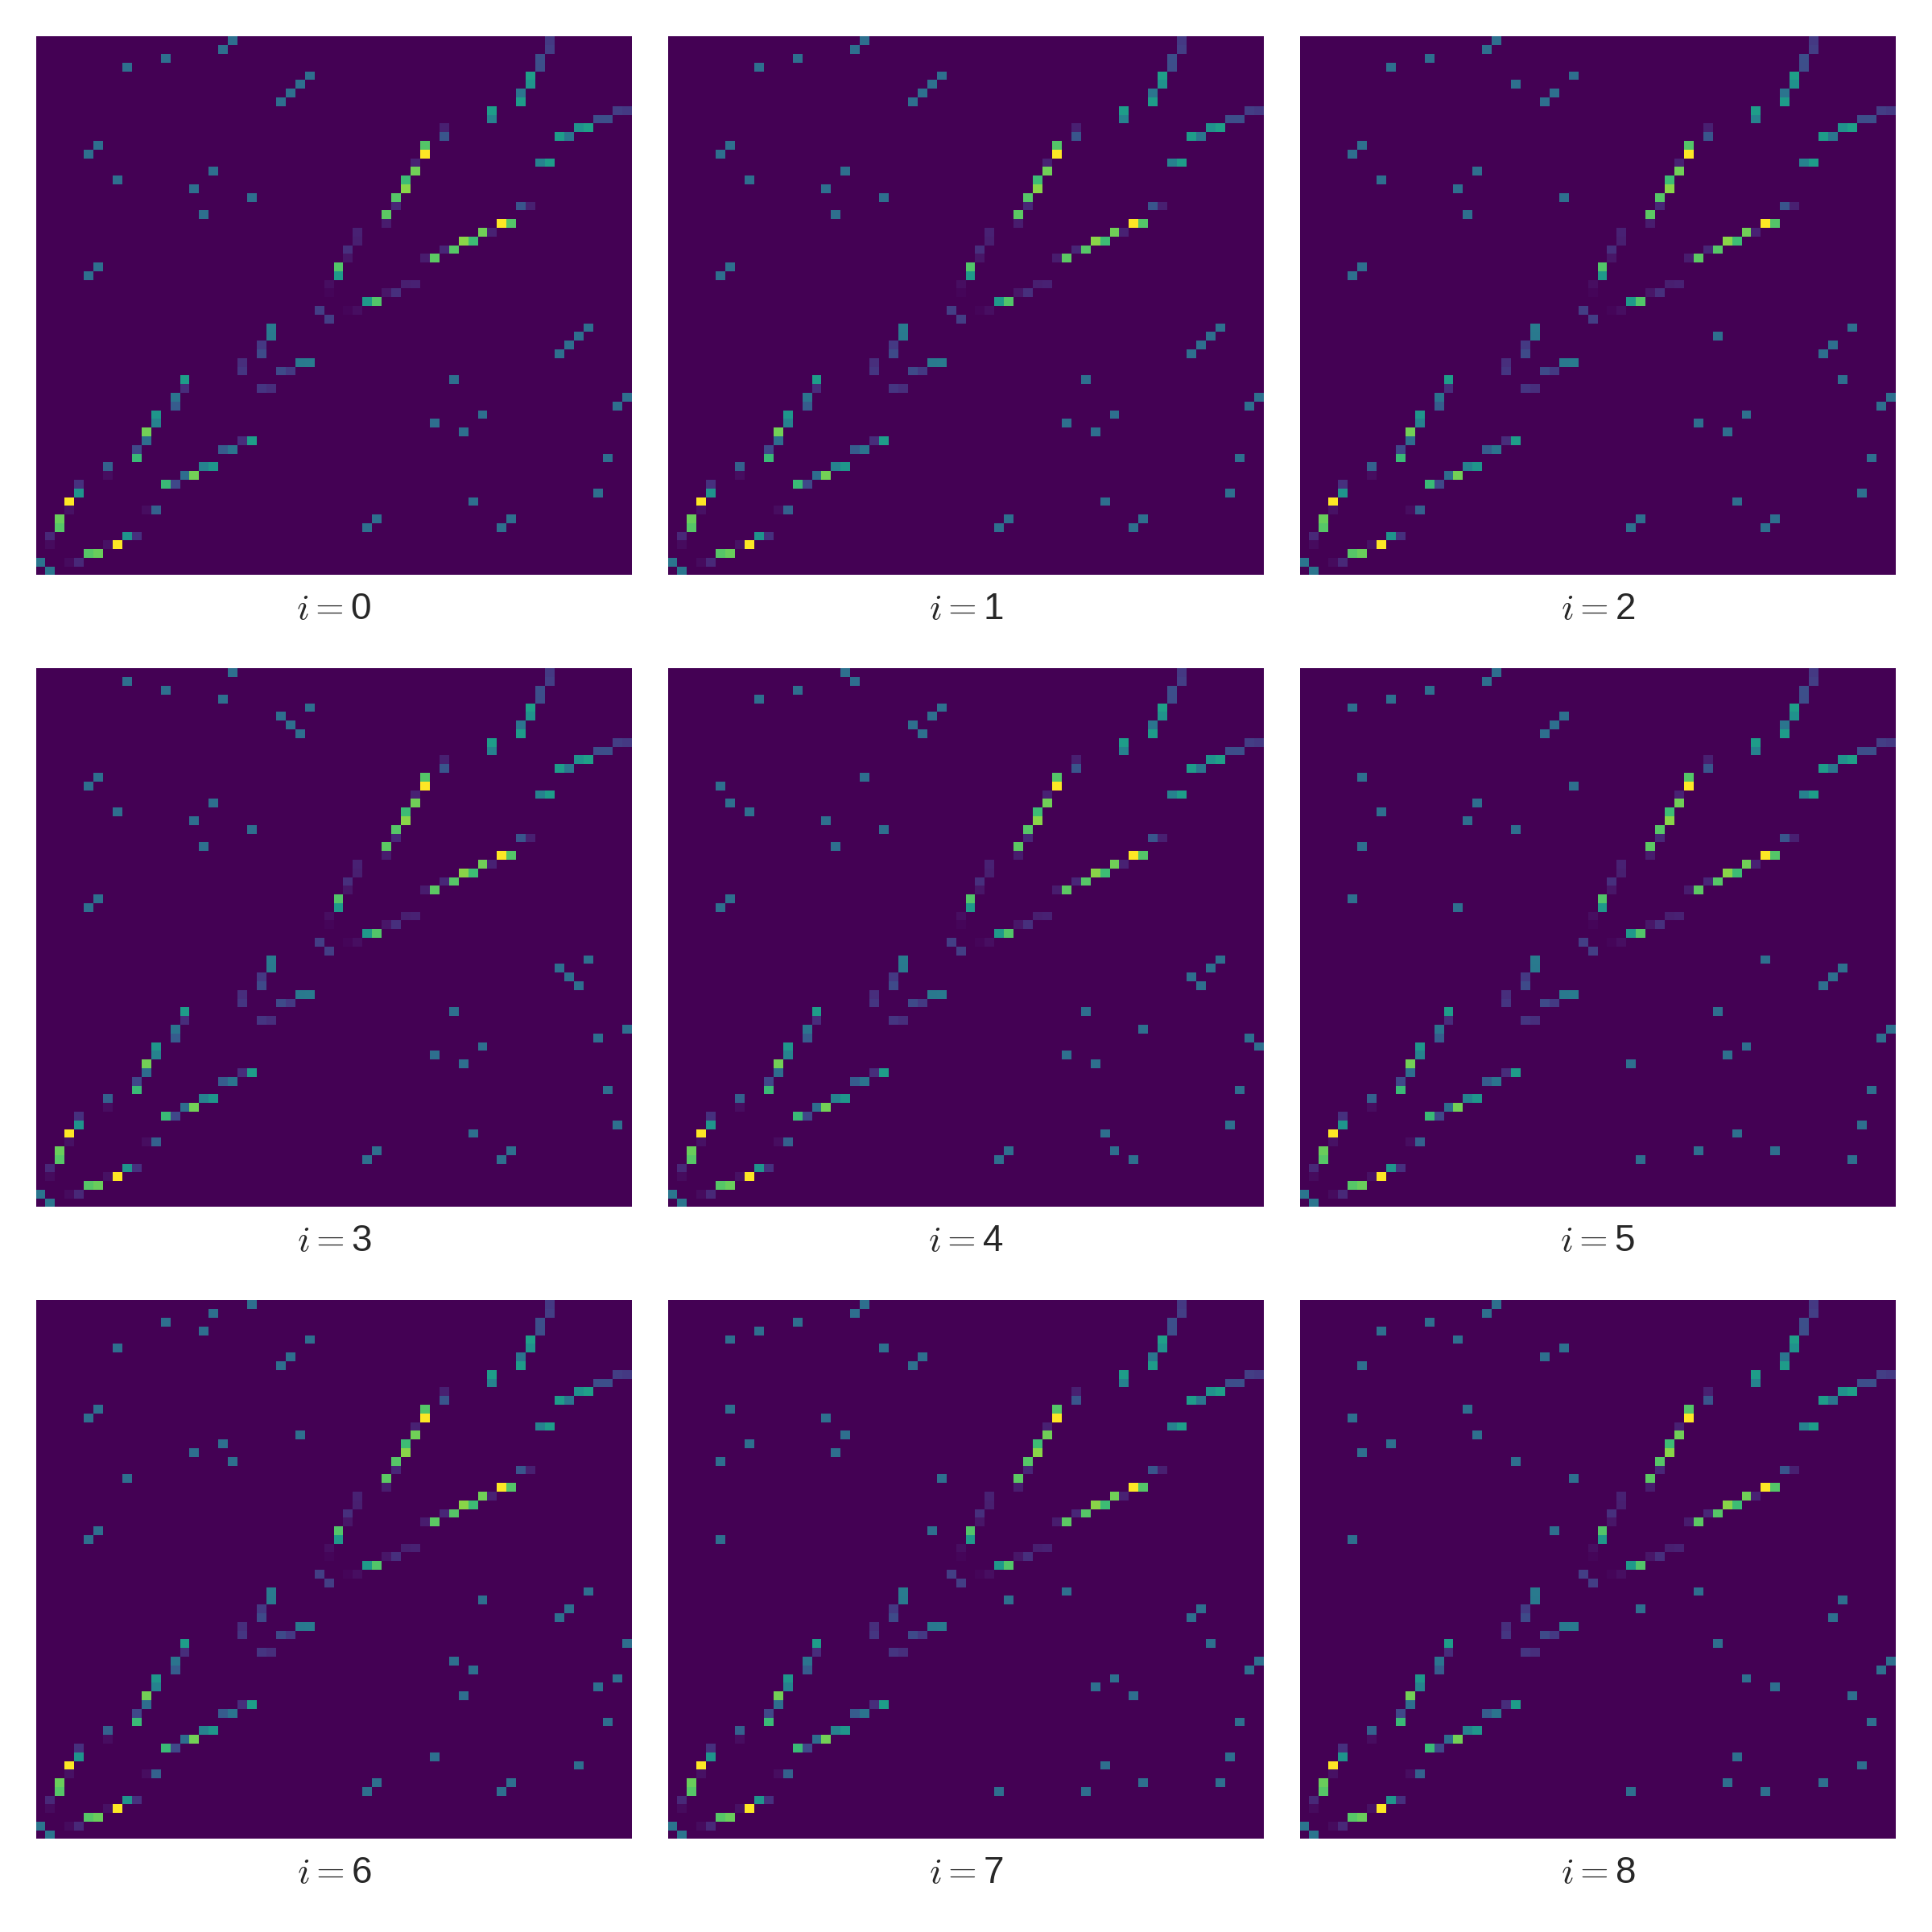
\includegraphics[width=\textwidth]{FishPoo/figures/gopher_louse_adjacency_permutations}
    \caption{Successive permutations from none ($i=0$) to eight ($i=8$) of the graph adjacency matrix of interactions among pocket gophers and their chewing lice parasites from Hafner {\em et al.} \cite{hafner1994disparate}. Permutations are carried out by swapping the associations of randomly chosen links in between the host and parasite tree. }
    \label{fig:FP_ajperm}
\end{figure}